\section{Results}

Our optimization reveals a sobering but nuanced picture of carbon pricing effectiveness in driving industrial decarbonization. The central finding is unambiguous: even aggressive carbon pricing aligned with Net Zero 2050 targets fails to keep POSCO's emissions within its climate-consistent carbon budget. However, the reasons for this failure—and the pathways the model does choose—provide crucial insights for policy design. We organize our findings around four questions: Do carbon prices drive emission reductions? Which technologies actually get deployed? Can any price trajectory achieve budget compliance? And what are the cost implications for competitiveness?

Before diving into details, Table~\ref{tab:scenario-comparison} provides a comprehensive overview of headline metrics across all three NGFS carbon price scenarios. This reference point helps contextualize the subsection-by-section analysis that follows.

\subsection{Carbon prices drive substantial but insufficient emission reductions}

Carbon pricing works—but not well enough. Figure~\ref{fig:scope1-by-scenario} shows how POSCO's annual Scope 1 emissions evolve under the three NGFS price trajectories, with the Net Zero 2050 (No CCUS) sensitivity highlighted for comparison. The emission reductions are dramatic: under the Net Zero pathway, annual emissions fall from 81 MtCO$_2$ in 2025 to just 23.1 MtCO$_2$ by 2050, a 71\% decline. The Below 2°C trajectory delivers less aggressive reductions, bottoming out at 53.3 MtCO$_2$ in 2050, while the NDC-consistent pricing barely moves the needle, with 2050 emissions plateauing at 71.1 MtCO$_2$.

\begin{figure}[!t]
  \centering
  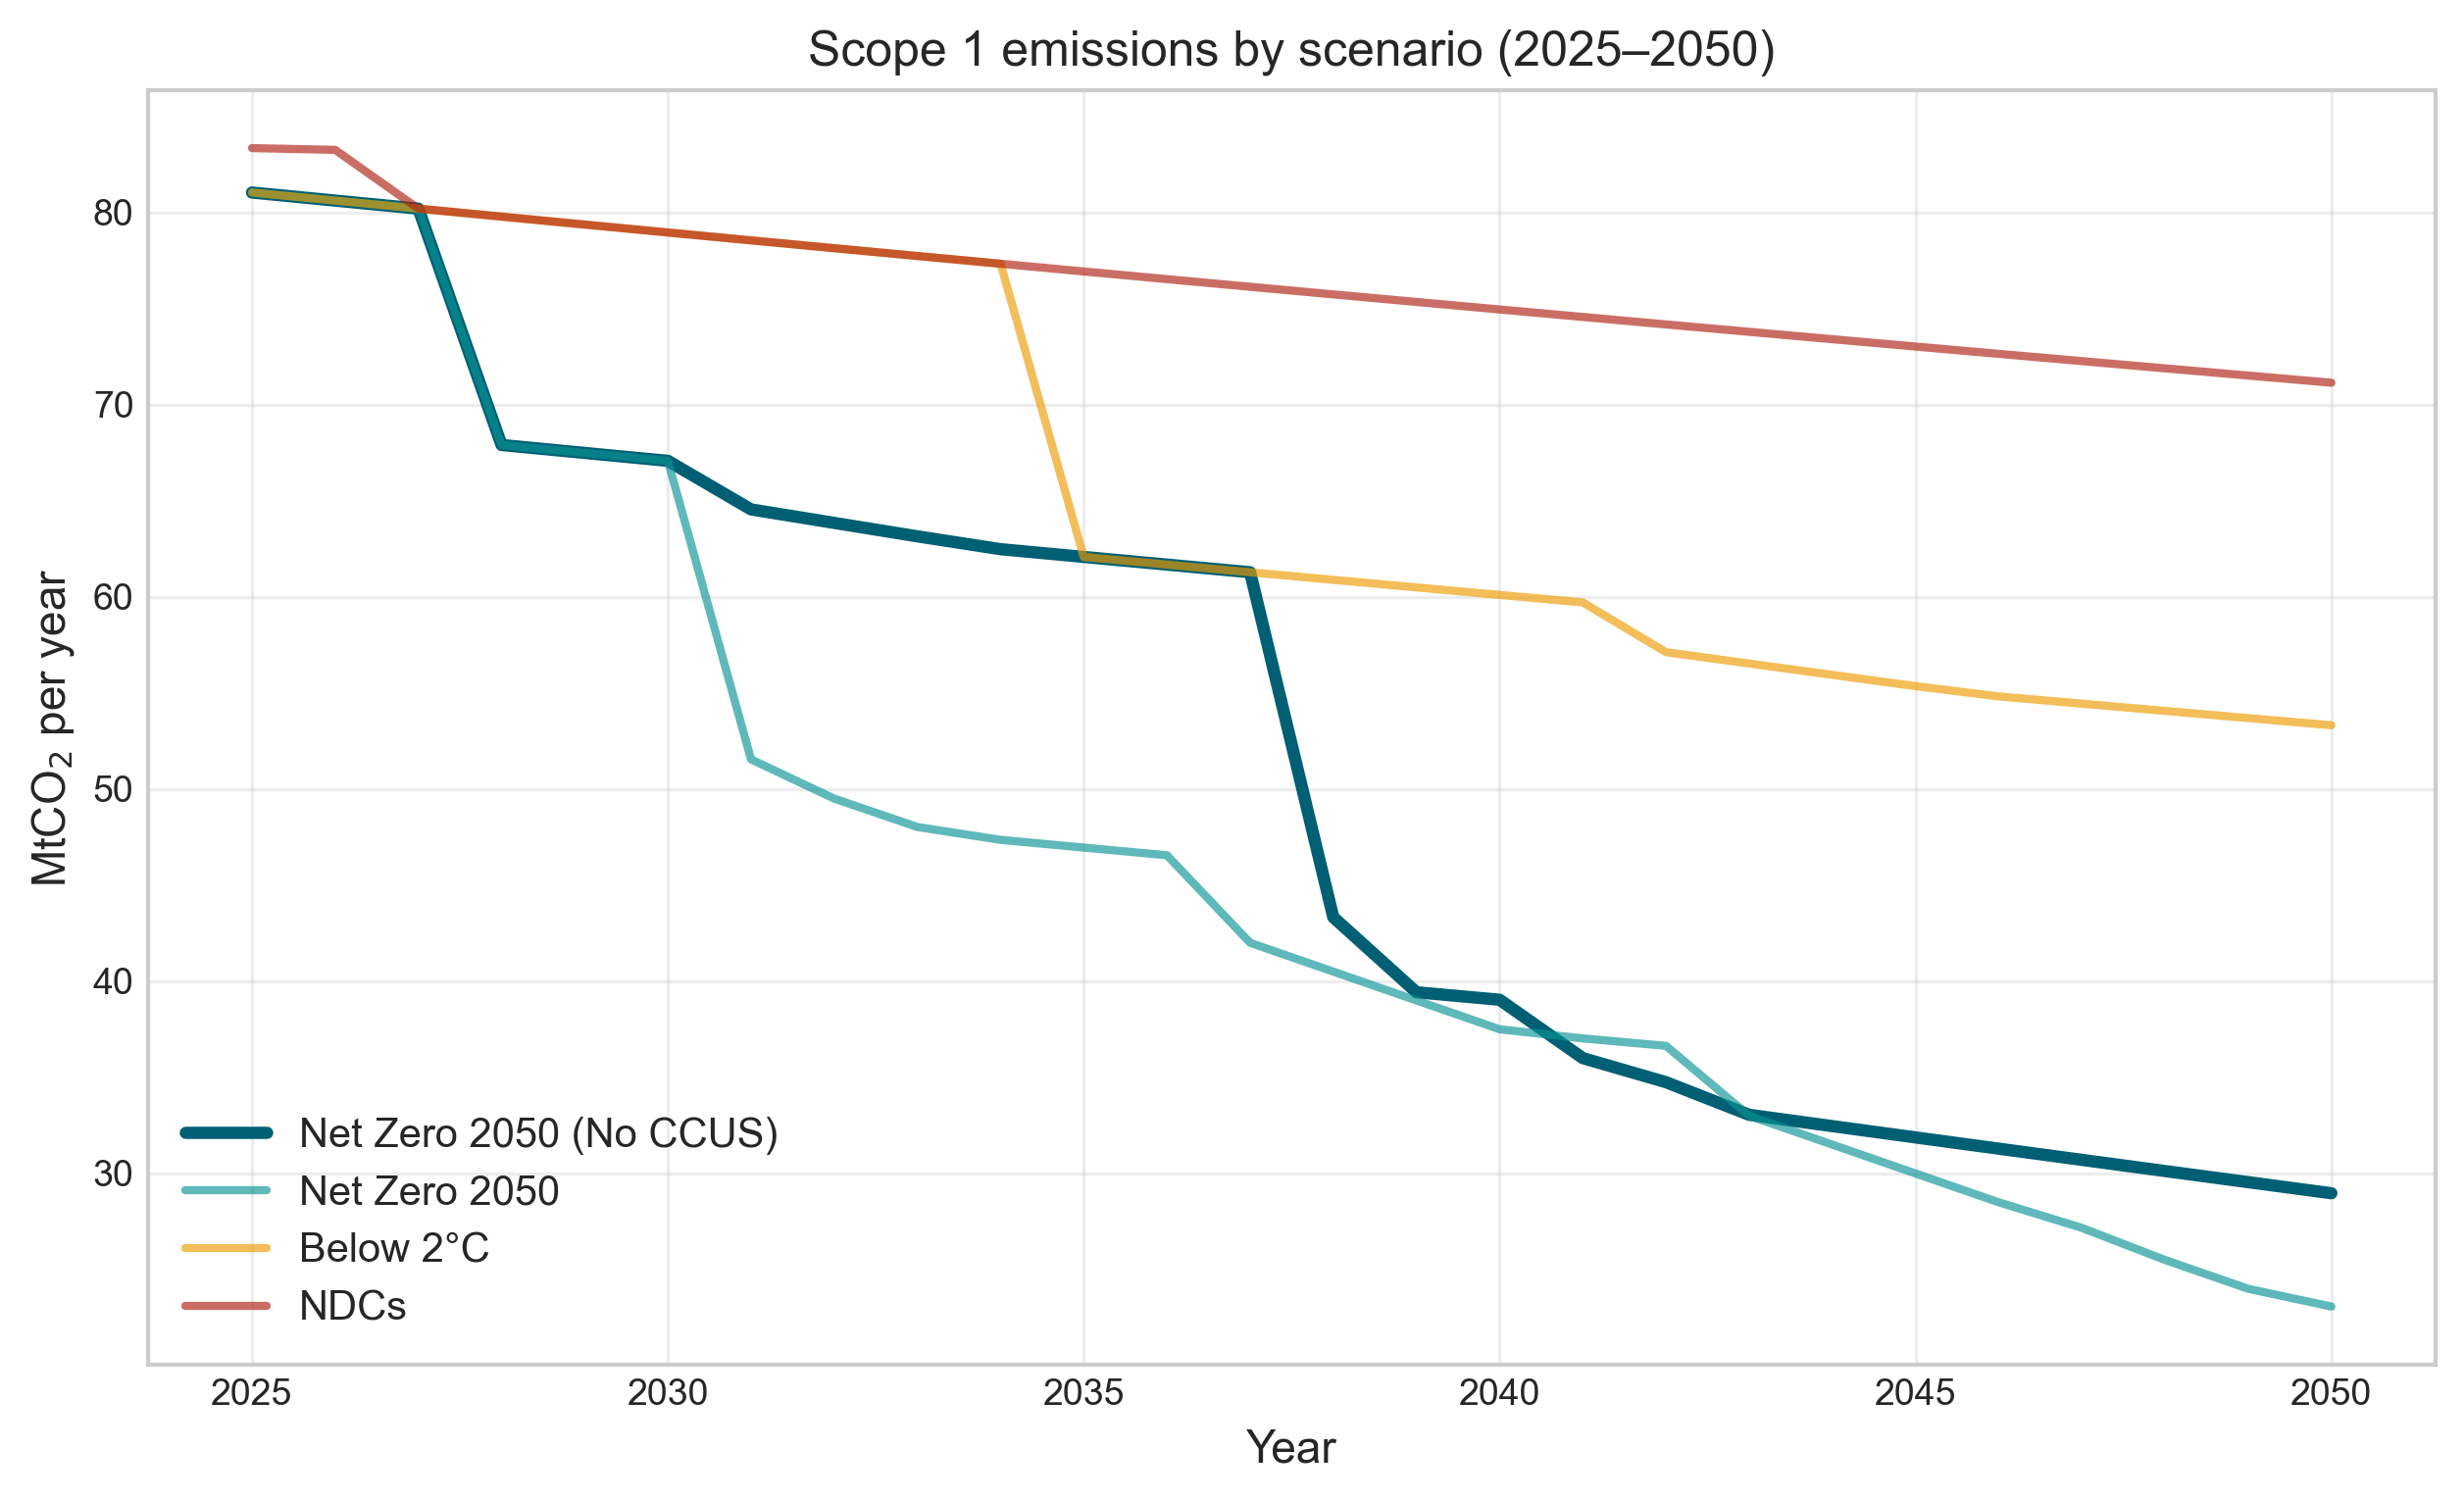
\includegraphics[width=0.8\linewidth]{scope1_by_scenario}
  \caption{Scope~1 emissions by scenario, including the Net Zero 2050 pathway with CCUS disabled (2025--2050).}
  \label{fig:scope1-by-scenario}
\end{figure}

These reductions matter enormously—the difference between NDC pricing and Net Zero pricing amounts to 791 MtCO$_2$ of avoided emissions over the planning horizon. Yet as we show in Section 4.3, even the most ambitious scenario still overshoots POSCO's allocated carbon budget. The price sensitivity is clear, but absolute price levels remain inadequate.

The No CCUS sensitivity reveals how dependent these pathways are on carbon capture technology. Removing CCUS availability while maintaining the same Net Zero price trajectory leaves emissions "stuck" above 45 MtCO$_2$ through the 2030s, declining only gradually to 29 MtCO$_2$ by 2050. This 26\% higher endpoint compared to the CCUS-enabled case underscores that carbon pricing alone cannot drive sufficient emission reductions if key abatement technologies remain unavailable or uneconomic. The model finds alternative routes—particularly hydrogen DRI, as we detail below—but these prove more expensive and still fail to close the budget gap entirely.

\subsection{Technology transitions follow sharp price thresholds, not gradual shifts}

One of our most striking findings is how technology deployment responds to discrete price thresholds rather than gradual carbon price increases. The model's investment behavior exhibits threshold effects that have important implications for policy predictability and investment timing.

Figure~\ref{fig:technology-transition} and Table~\ref{tab:annual-shares-ngfs_netzero2050} show that scrap-based EAF deployment remains essentially frozen—locked at just 4.5\% of total output—while carbon prices stay below \$100/tCO$_2$. Then, once the Net Zero pathway crosses \$110/tCO$_2$ in 2028, scrap-EAF share jumps suddenly to 22.8\% as the model builds a single 9 Mt capacity tranche. This discrete jump reflects the lumpy nature of steel industry investment: POSCO cannot gradually expand scrap-EAF capacity because it must construct entirely new facilities from scratch. The company's current operations are almost exclusively blast-furnace based, with only 1.7 Mt/y of specialty stainless EAF assets that cannot substitute for automotive-grade flat products \citep{POSCO2023SR}. Building EAF capacity means greenfield investment in complete production modules.

\begin{figure}[!t]
  \centering
  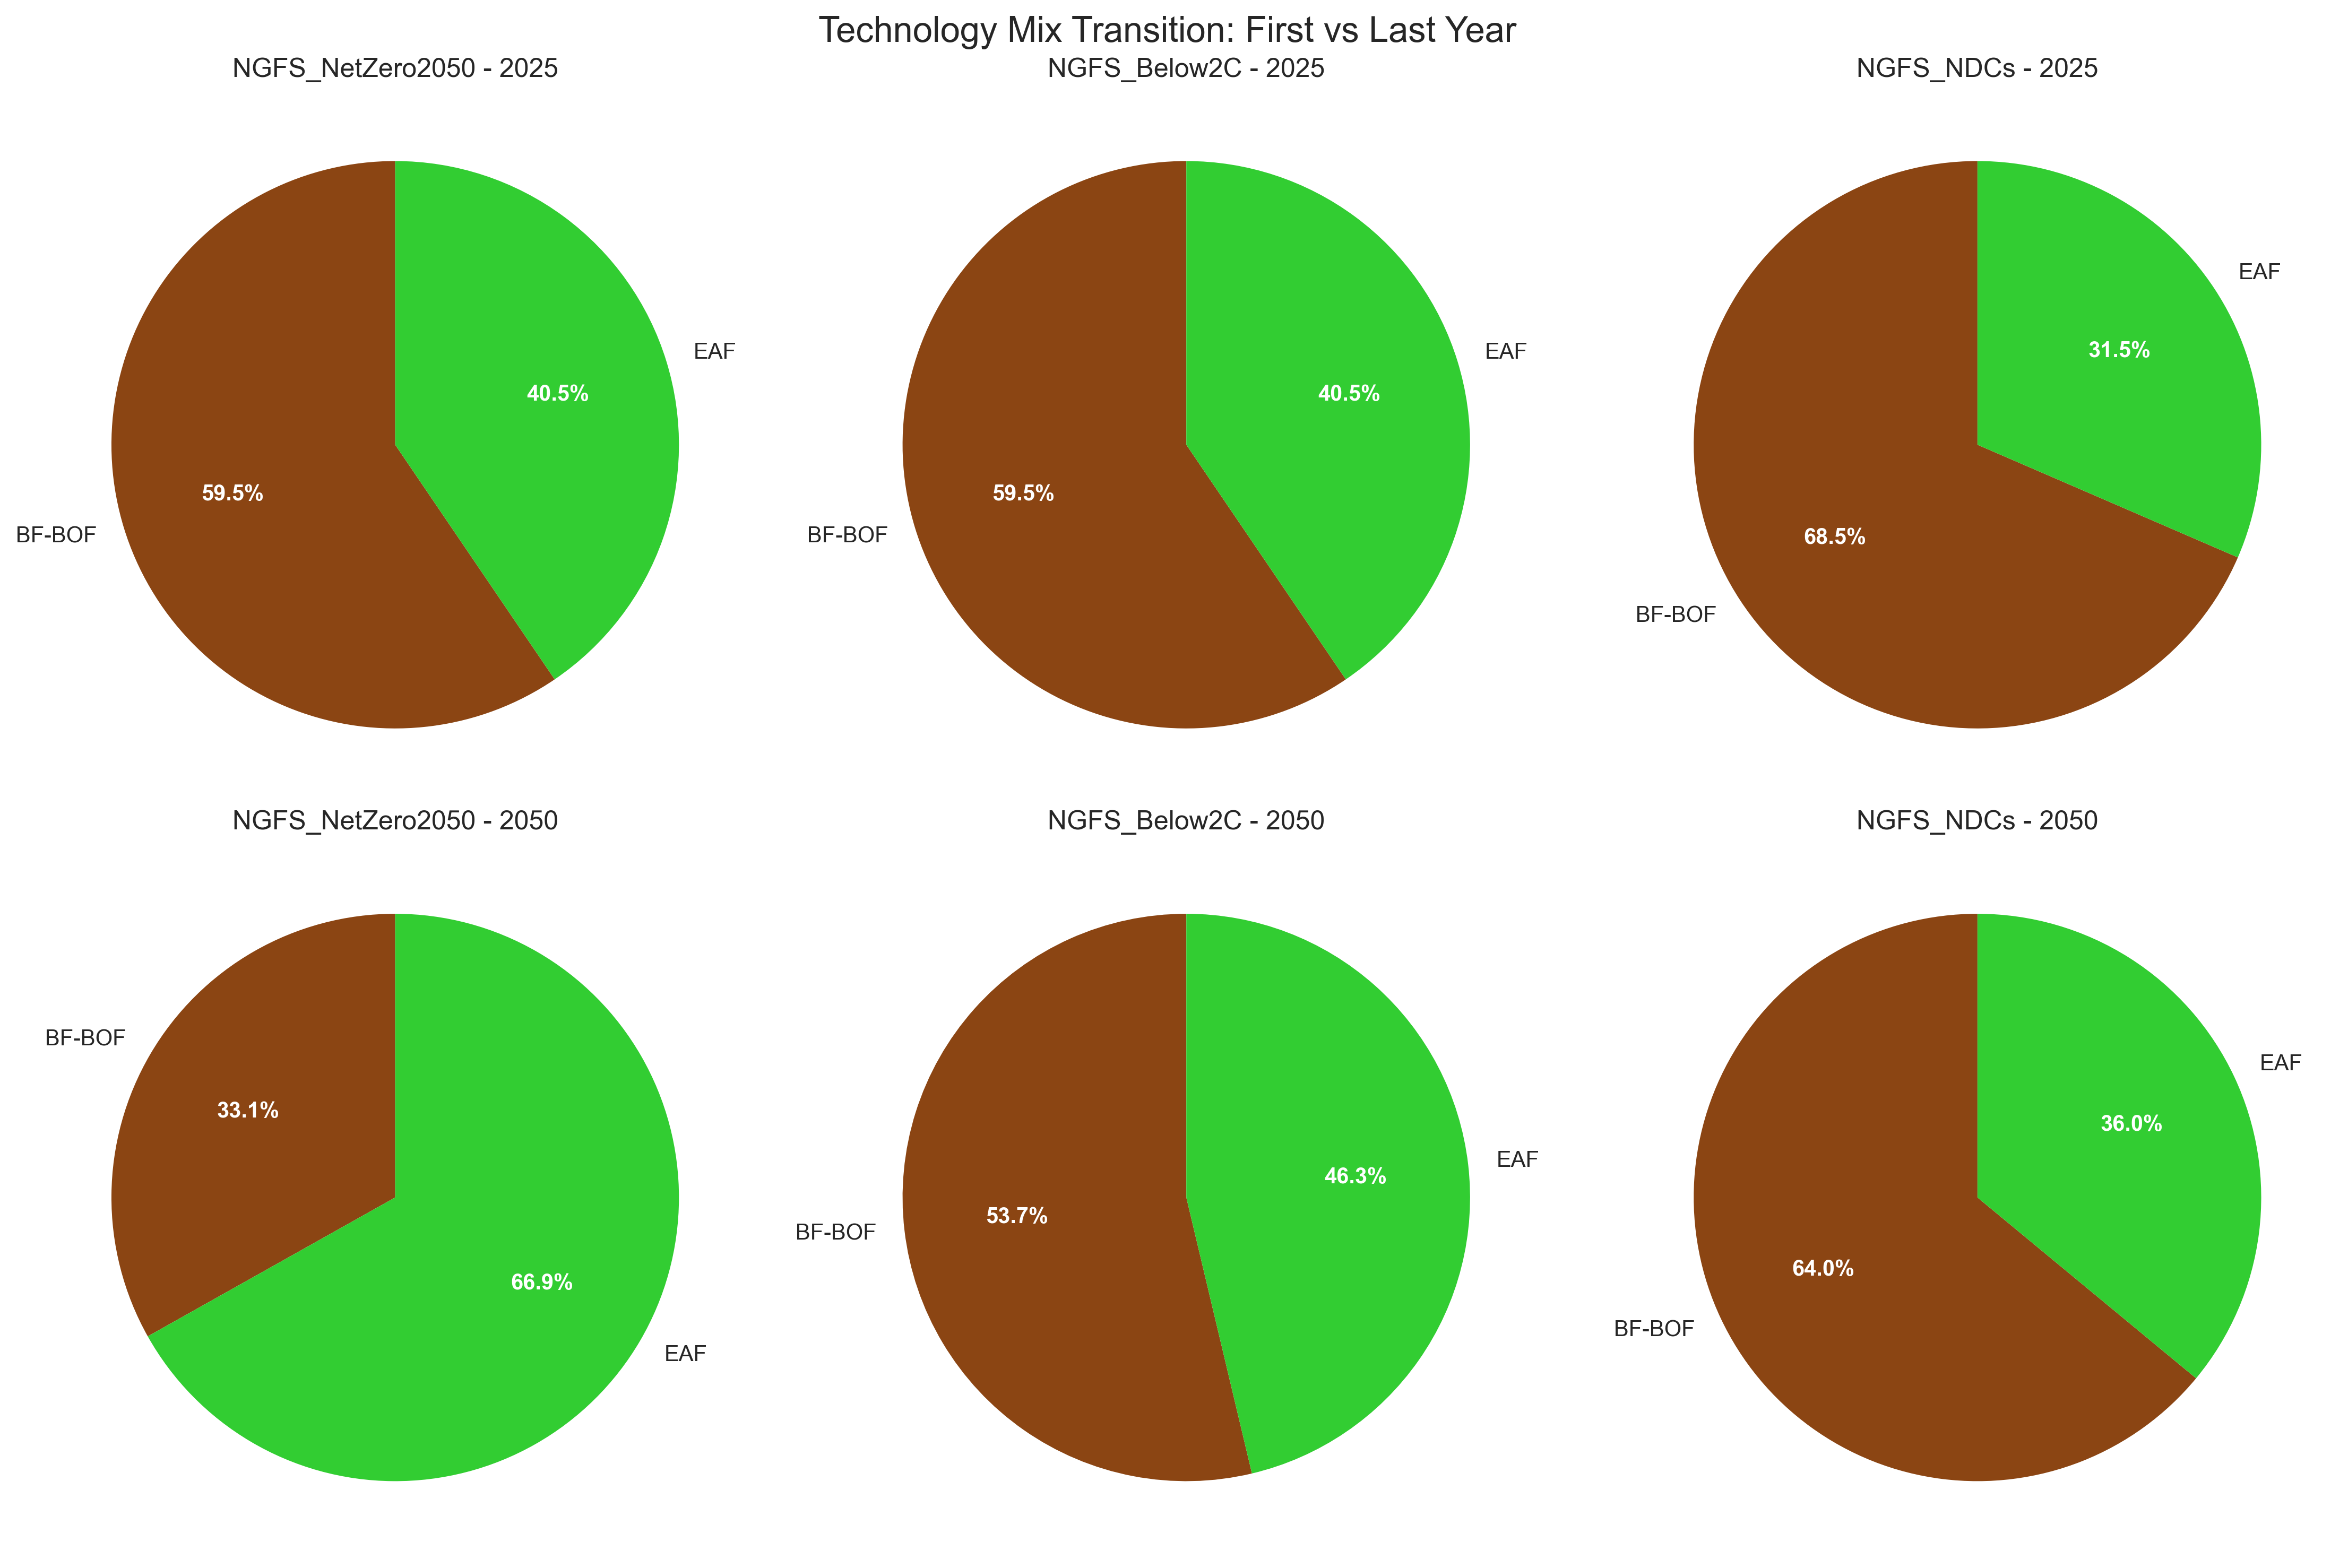
\includegraphics[width=0.8\linewidth]{technology_transition}
  \caption{Technology shares by scenario. The top panel emphasizes the Net Zero 2050 pathway with CCUS disabled; lower panels show the NGFS Net Zero, Below~2$^\circ$C, and NDC trajectories.}
  \label{fig:technology-transition}
\end{figure}

\begin{figure}[!t]
  \centering
  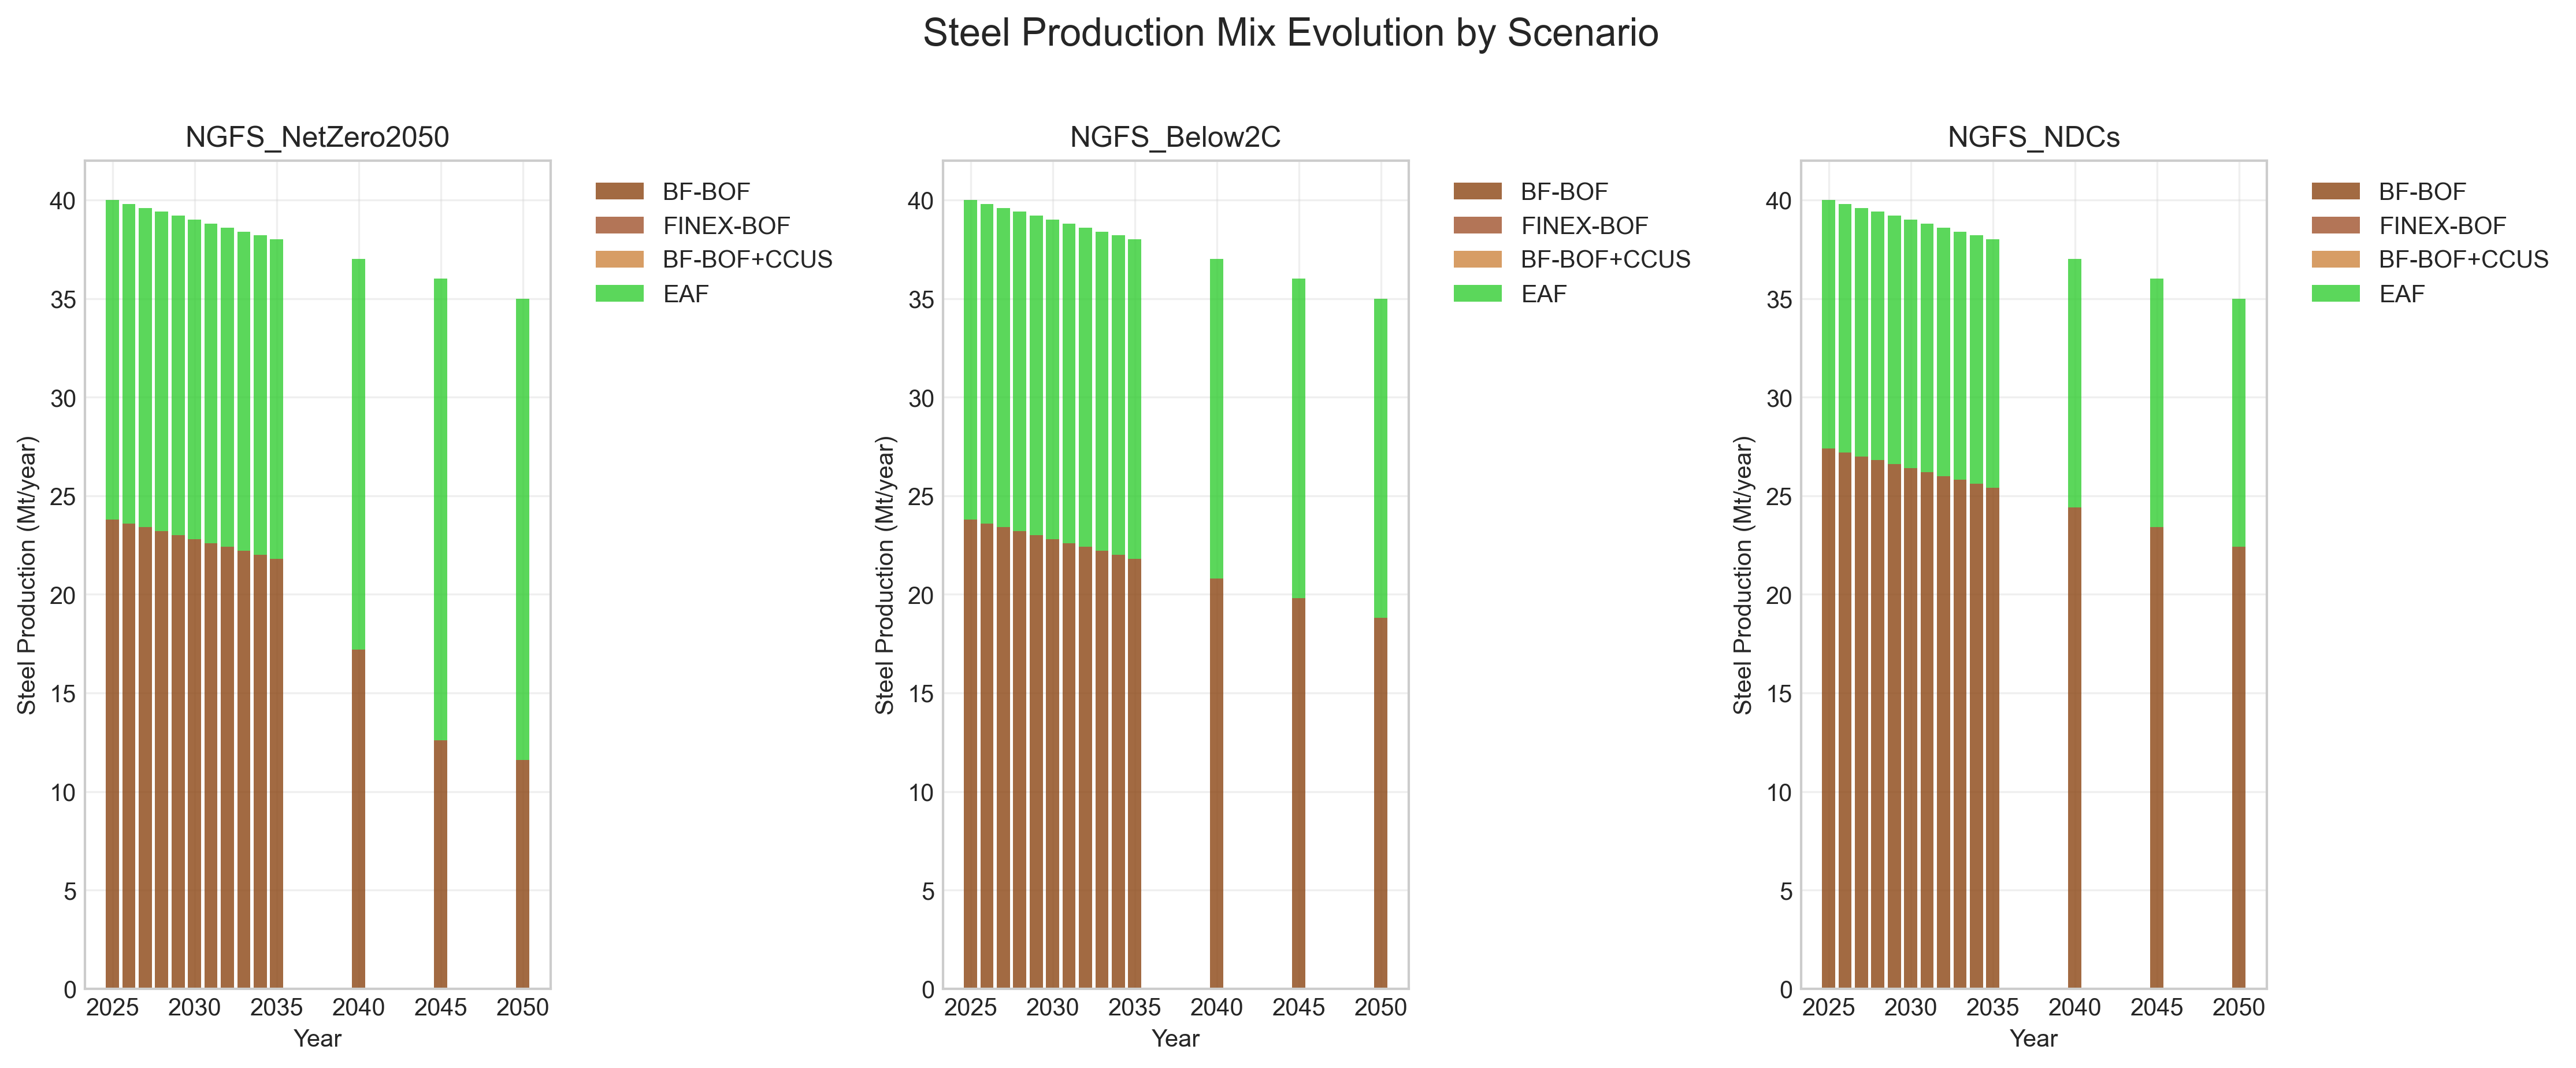
\includegraphics[width=0.8\linewidth]{production_mix_evolution}
  \caption{Production mix by technology route (Mt/year). Panels mirror Figure~\ref{fig:technology-transition}, with the Net Zero 2050 (No CCUS) case highlighted.}
  \label{fig:production-mix}
\end{figure}

Scrap availability then caps further EAF expansion at 35.7\% of output even under the most aggressive carbon prices. This ceiling reflects Korea's structural scrap deficit—unlike scrap-rich markets such as the United States, Korea must import substantial quantities of high-quality scrap to supply EAF operations. The binding constraint is not capital cost or carbon price, but physical feedstock availability.

Carbon capture exhibits similar threshold behavior but at even higher price levels. CCUS retrofits enter the portfolio only after carbon prices reach \$165/tCO$_2$ in 2031. At that point, the model retrofits one 9 Mt blast furnace module with capture equipment. Subsequent price increases to \$225/tCO$_2$ and \$255/tCO$_2$ trigger additional retrofits until CCUS-equipped furnaces supply 51\% of 2050 production under the Net Zero pathway. The economics are straightforward: CCUS retrofits carry a 65\% capital cost premium over conventional blast furnaces, requiring carbon prices above \$165/tCO$_2$ to justify the investment.

Lower price trajectories never activate carbon capture at all. The Below 2°C pathway peaks at \$240/tCO$_2$—high, but not quite high enough to justify widespread CCUS deployment. As a result, 64\% of output in 2050 remains unabated blast furnaces under this scenario. The NDC ceiling of \$100/tCO$_2$ fails to justify any structural technology change, keeping the BF-BOF share above 95\% throughout the entire planning horizon (see Tables~\ref{tab:annual-shares-ngfs_below2c} and \ref{tab:annual-shares-ngfs_ndcs}).

The policy implication is clear: if policymakers want to trigger low-carbon technology deployment, they need carbon prices sustained well above \$150/tCO$_2$—not just peak prices, but sustained multi-decade trajectories. Gradual price increases that never cross critical thresholds will not drive transformation.

Perhaps most revealing is what the model does not choose. Hydrogen-based direct reduction, natural gas DRI, and POSCO's proprietary FINEX technology remain dormant across all scenarios, even at carbon prices reaching \$450/tCO$_2$. The reason is straightforward: at our baseline hydrogen cost assumptions (\$4.5/kg in 2030, declining to \$2.5/kg by 2050), hydrogen routes simply cannot compete economically with the CCUS-plus-scrap combination. Our cost assumptions align with major techno-economic assessments \citep{MaterialEconomics2019,demailly2018european}, which estimate that hydrogen steel requires delivered hydrogen below \$2.0-2.5/kg to reach cost parity with conventional routes—a threshold our baseline trajectory barely approaches by 2050.

This finding challenges narratives that position hydrogen as the primary decarbonization pathway for steel. Under realistic cost assumptions and within the 2025-2050 timeframe, carbon pricing alone cannot make hydrogen competitive. Only when we disable CCUS entirely (discussed in Section 4.6) does the model reluctantly turn to hydrogen DRI—and even then, the outcome is worse on both emissions and costs.

\subsection{All carbon price trajectories overshoot the sectoral budget—even Net Zero}

We now confront the central research question: can carbon pricing drive investment decisions that remain within climate-consistent carbon budgets? The answer is unequivocal: no. Figure~\ref{fig:emissions-pathways} and our cumulative emission calculations reveal systematic budget overshoots across all scenarios.

\begin{figure}[!t]
  \centering
  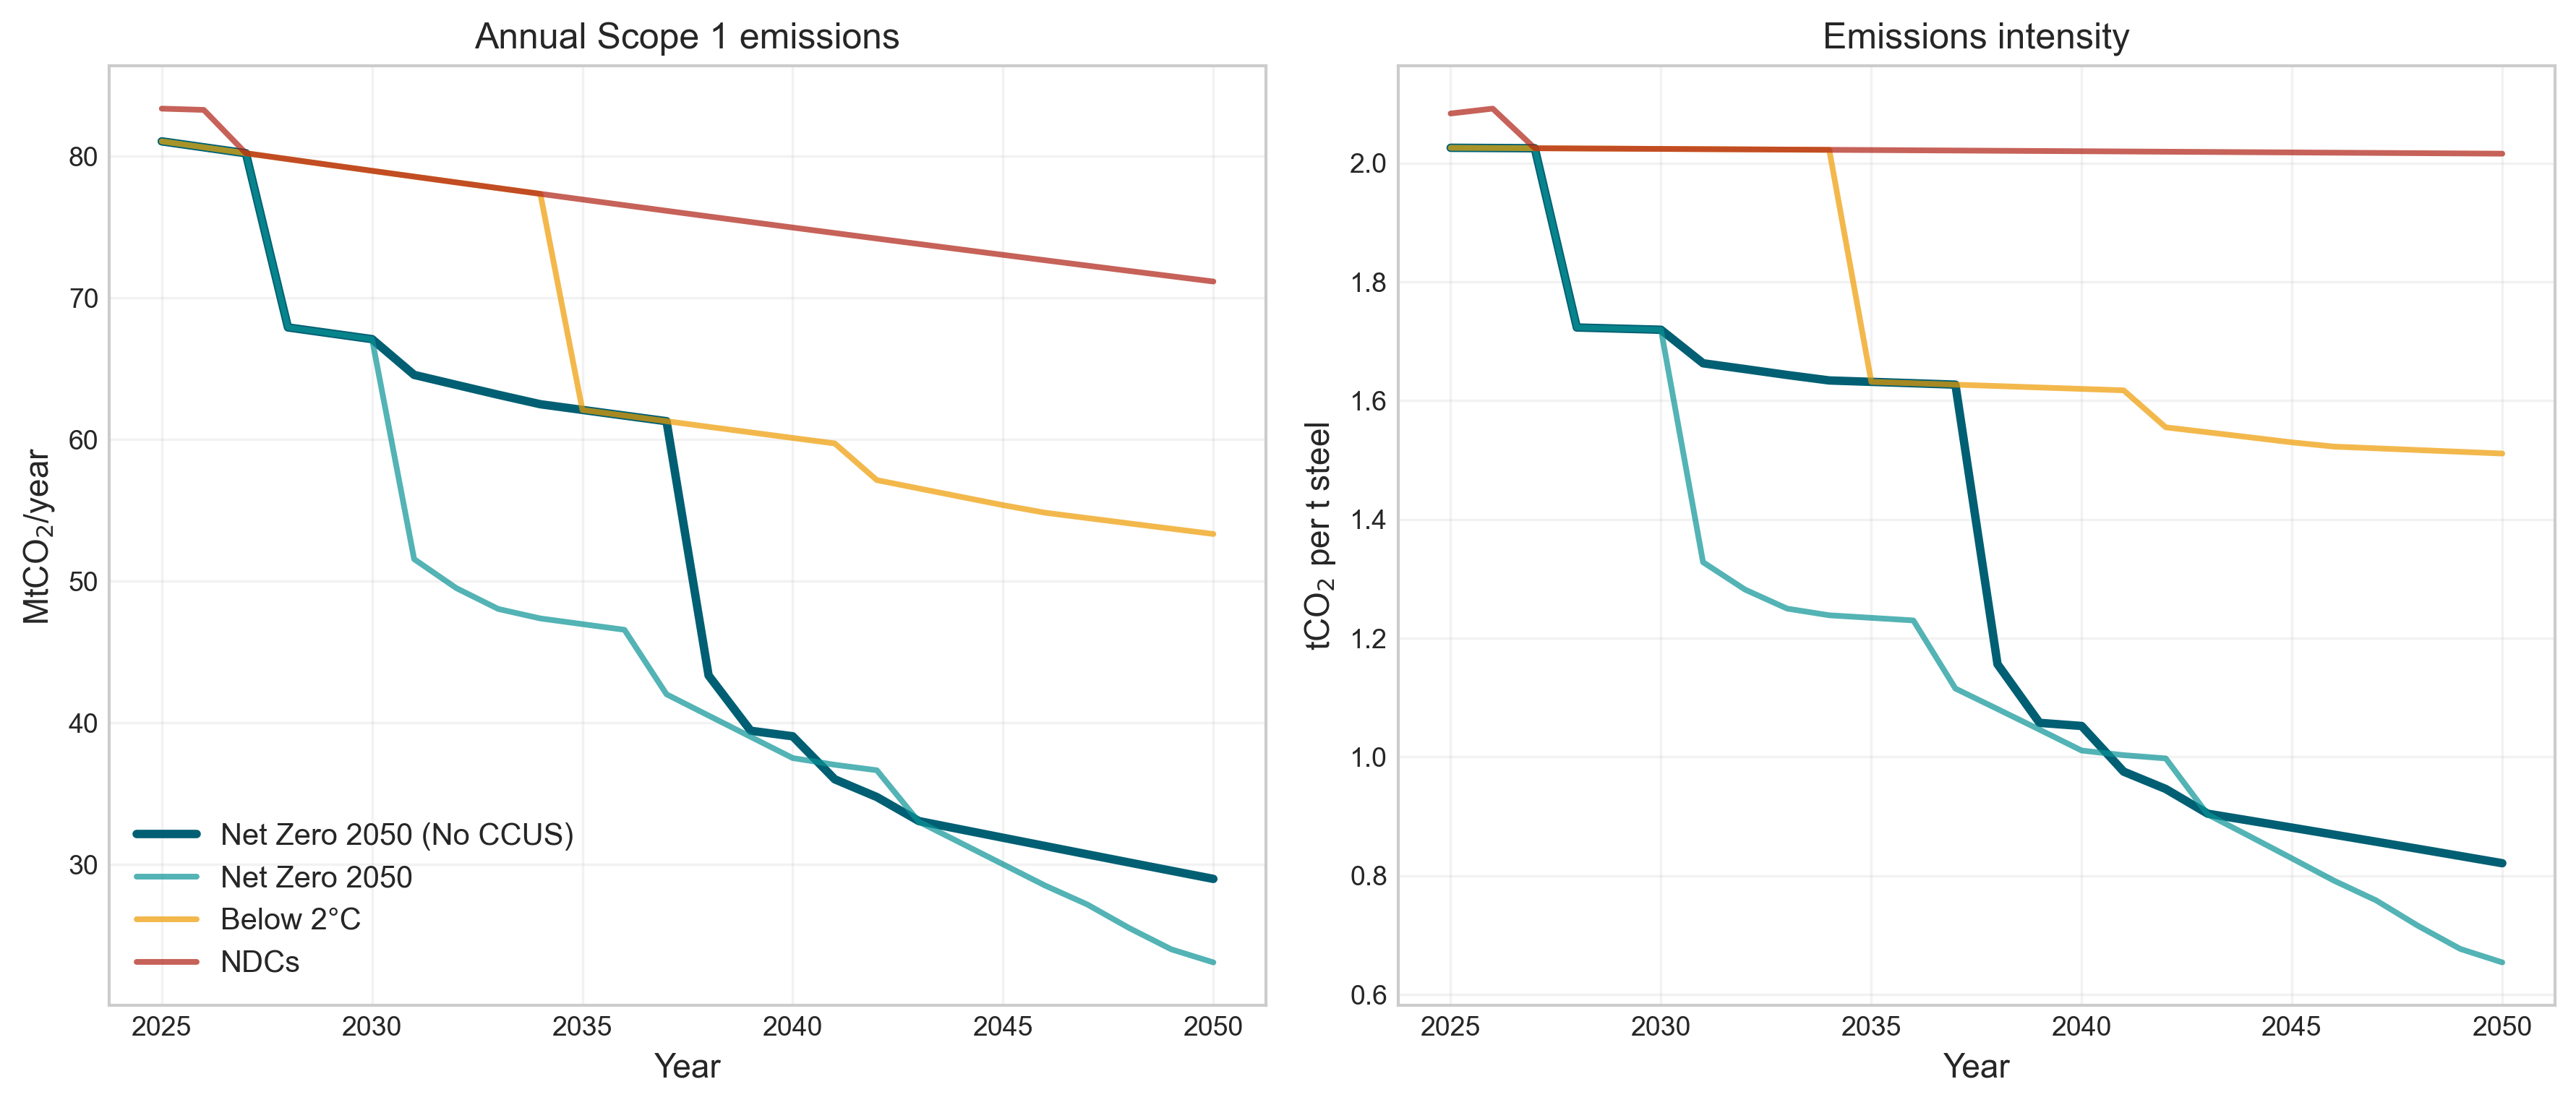
\includegraphics[width=0.85\linewidth]{emissions_pathways}
  \caption{Annual Scope~1 emissions (left) and emissions intensity (right) by scenario.}
  \label{fig:emissions-pathways}
\end{figure}

Integrating annual emissions over the 2025-2050 period produces cumulative totals of 1,190 MtCO$_2$ under Net Zero pricing, 1,713 MtCO$_2$ under Below 2°C, and 1,981 MtCO$_2$ in the NDC case. Compared with POSCO's allocated carbon budget of 1,110 MtCO$_2$ (derived in Section 3.3), the overshoots are:

\begin{itemize}[leftmargin=*]
  \item \textbf{Net Zero 2050:} +80 MtCO$_2$ (+7.2\%)
  \item \textbf{Below 2°C:} +603 MtCO$_2$ (+54\%)
  \item \textbf{NDCs:} +871 MtCO$_2$ (+78\%)
\end{itemize}

Let us put these numbers in perspective. The Below 2°C overshoot of 603 MtCO$_2$ represents more than half the entire allocated budget—POSCO would need to cut an additional 35\% from its optimized emission pathway to achieve compliance. The NDC overshoot of 871 MtCO$_2$ is simply catastrophic from a climate perspective, representing nearly 80\% excess emissions above the budget.

Even the most ambitious Net Zero scenario overshoots by 80 MtCO$_2$, or 7.2\%. This residual gap is particularly revealing because it persists despite carbon prices reaching \$450/tCO$_2$ by 2050—levels far beyond anything currently implemented in carbon markets globally. The implication is that budget compliance would require either carbon prices rising well above \$450/tCO$_2$ in later periods, or complementary policies that constrain production or mandate specific technologies beyond what price signals alone can deliver.

The cumulative gap maps directly onto a carbon price gap. Moving from the NDC ceiling (\$100/tCO$_2$) to the Net Zero peak (\$450/tCO$_2$) yields a 791 MtCO$_2$ reduction—implying that each additional \$100/tCO$_2$ of carbon price drives roughly 226 MtCO$_2$ of cumulative abatement over the planning horizon. The residual 80 MtCO$_2$ shortfall under Net Zero would require sustained prices above \$500/tCO$_2$ to close entirely through carbon pricing alone.

Free allocation exacerbates this problem substantially. Even under the Net Zero pathway, only 72 MtCO$_2$ of cumulative emissions face actual ETS liability—just 6\% of total emissions. The Below 2°C pathway pays for only 596 MtCO$_2$ out of 1,713 MtCO$_2$ emitted (35\%), while the NDC case sees 863 MtCO$_2$ of net ETS-liable emissions (44\%). This means that most emissions remain effectively unpriced despite rising nominal carbon prices, because free allocation shields firms from marginal carbon costs.

Closing the residual budget gap under Net Zero therefore requires one of two interventions: either a sharper price floor escalation after 2040 that drives prices well above \$500/tCO$_2$, or a much faster phase-down of free allocation so that firms internalize full carbon costs before the next blast furnace relining cycle in the early 2030s. Without addressing free allocation, even extremely high nominal carbon prices will continue to undershoot climate targets. Detailed budget compliance calculations are provided in the supplementary data file \texttt{outputs/analysis/carbon\_budget\_compliance.csv}.

Figure~\ref{fig:emissions-pathways} shows that only the NGFS Net Zero pathways materially shift emissions intensity below 1.0 tCO$_2$/t steel by 2050. The No CCUS sensitivity keeps intensity stubbornly above 0.8 tCO$_2$/t even in 2050, reflecting continued reliance on hydrogen DRI and residual unabated blast furnaces. This emissions intensity comparison reinforces that transforming the steel sector requires not just incremental improvements but wholesale technology replacement—exactly the kind of lumpy, expensive transitions that carbon pricing struggles to trigger without extremely high and sustained price signals.

\subsection{Higher carbon prices reduce total costs by substituting capital for compliance}

A counterintuitive but important finding emerges when we examine total system costs: more ambitious carbon pricing actually lowers lifetime costs rather than raising them. This result challenges common industry narratives that higher carbon prices necessarily harm competitiveness and profitability.

Summing undiscounted expenditure over the entire 2025-2050 period, the Net Zero pathway delivers the lowest lifetime system cost at \$791 billion, compared to \$871 billion for Below 2°C and \$842 billion for the NDC case. Dividing by cumulative steel output (978 Mt over the period) yields average costs of \$810/t under Net Zero, \$891/t under Below 2°C, and \$861/t in the NDC scenario.

At first glance, this seems paradoxical—how can higher carbon prices reduce costs? The mechanism is straightforward: ambitious pricing allows firms to substitute upfront capital investment in low-carbon technologies for recurring carbon compliance payments. Under the NDC trajectory, carbon prices remain low (\$100/tCO$_2$ ceiling), which means technologies like CCUS never become cost-justified. The firm therefore continues operating conventional blast furnaces and pays recurring ETS fees year after year. These compliance costs accumulate to \$59.7 billion over the planning horizon, representing 7.1\% of lifetime expenditure.

By contrast, Net Zero pricing justifies major CCUS retrofits and scrap-EAF expansion in the 2030s. While these investments carry high upfront capital costs, they dramatically reduce ongoing carbon liabilities. Total emissions under Net Zero reach 1,190 MtCO$_2$, but only 72 MtCO$_2$ face ETS liability after accounting for free allocation. This trims total compliance payments to just \$9.3 billion—merely 1.2\% of lifetime costs. The firm redirects cash flow from recurring carbon fees toward productive capital investment that permanently lowers emissions.

Table~\ref{tab:cost-abatement} quantifies this trade-off using marginal abatement cost metrics. Moving from the NDC baseline to Net Zero actually shows negative abatement costs of \$64/tCO$_2$—meaning the firm saves money while reducing emissions. The intermediate Below 2°C pathway requires positive \$108/tCO$_2$ in incremental support because carbon prices peak too early (\$240/tCO$_2$) to justify full CCUS deployment, leaving the firm in an awkward middle ground where it invests in partial decarbonization but still pays substantial carbon fees.

\begin{figure}[!t]
  \centering
  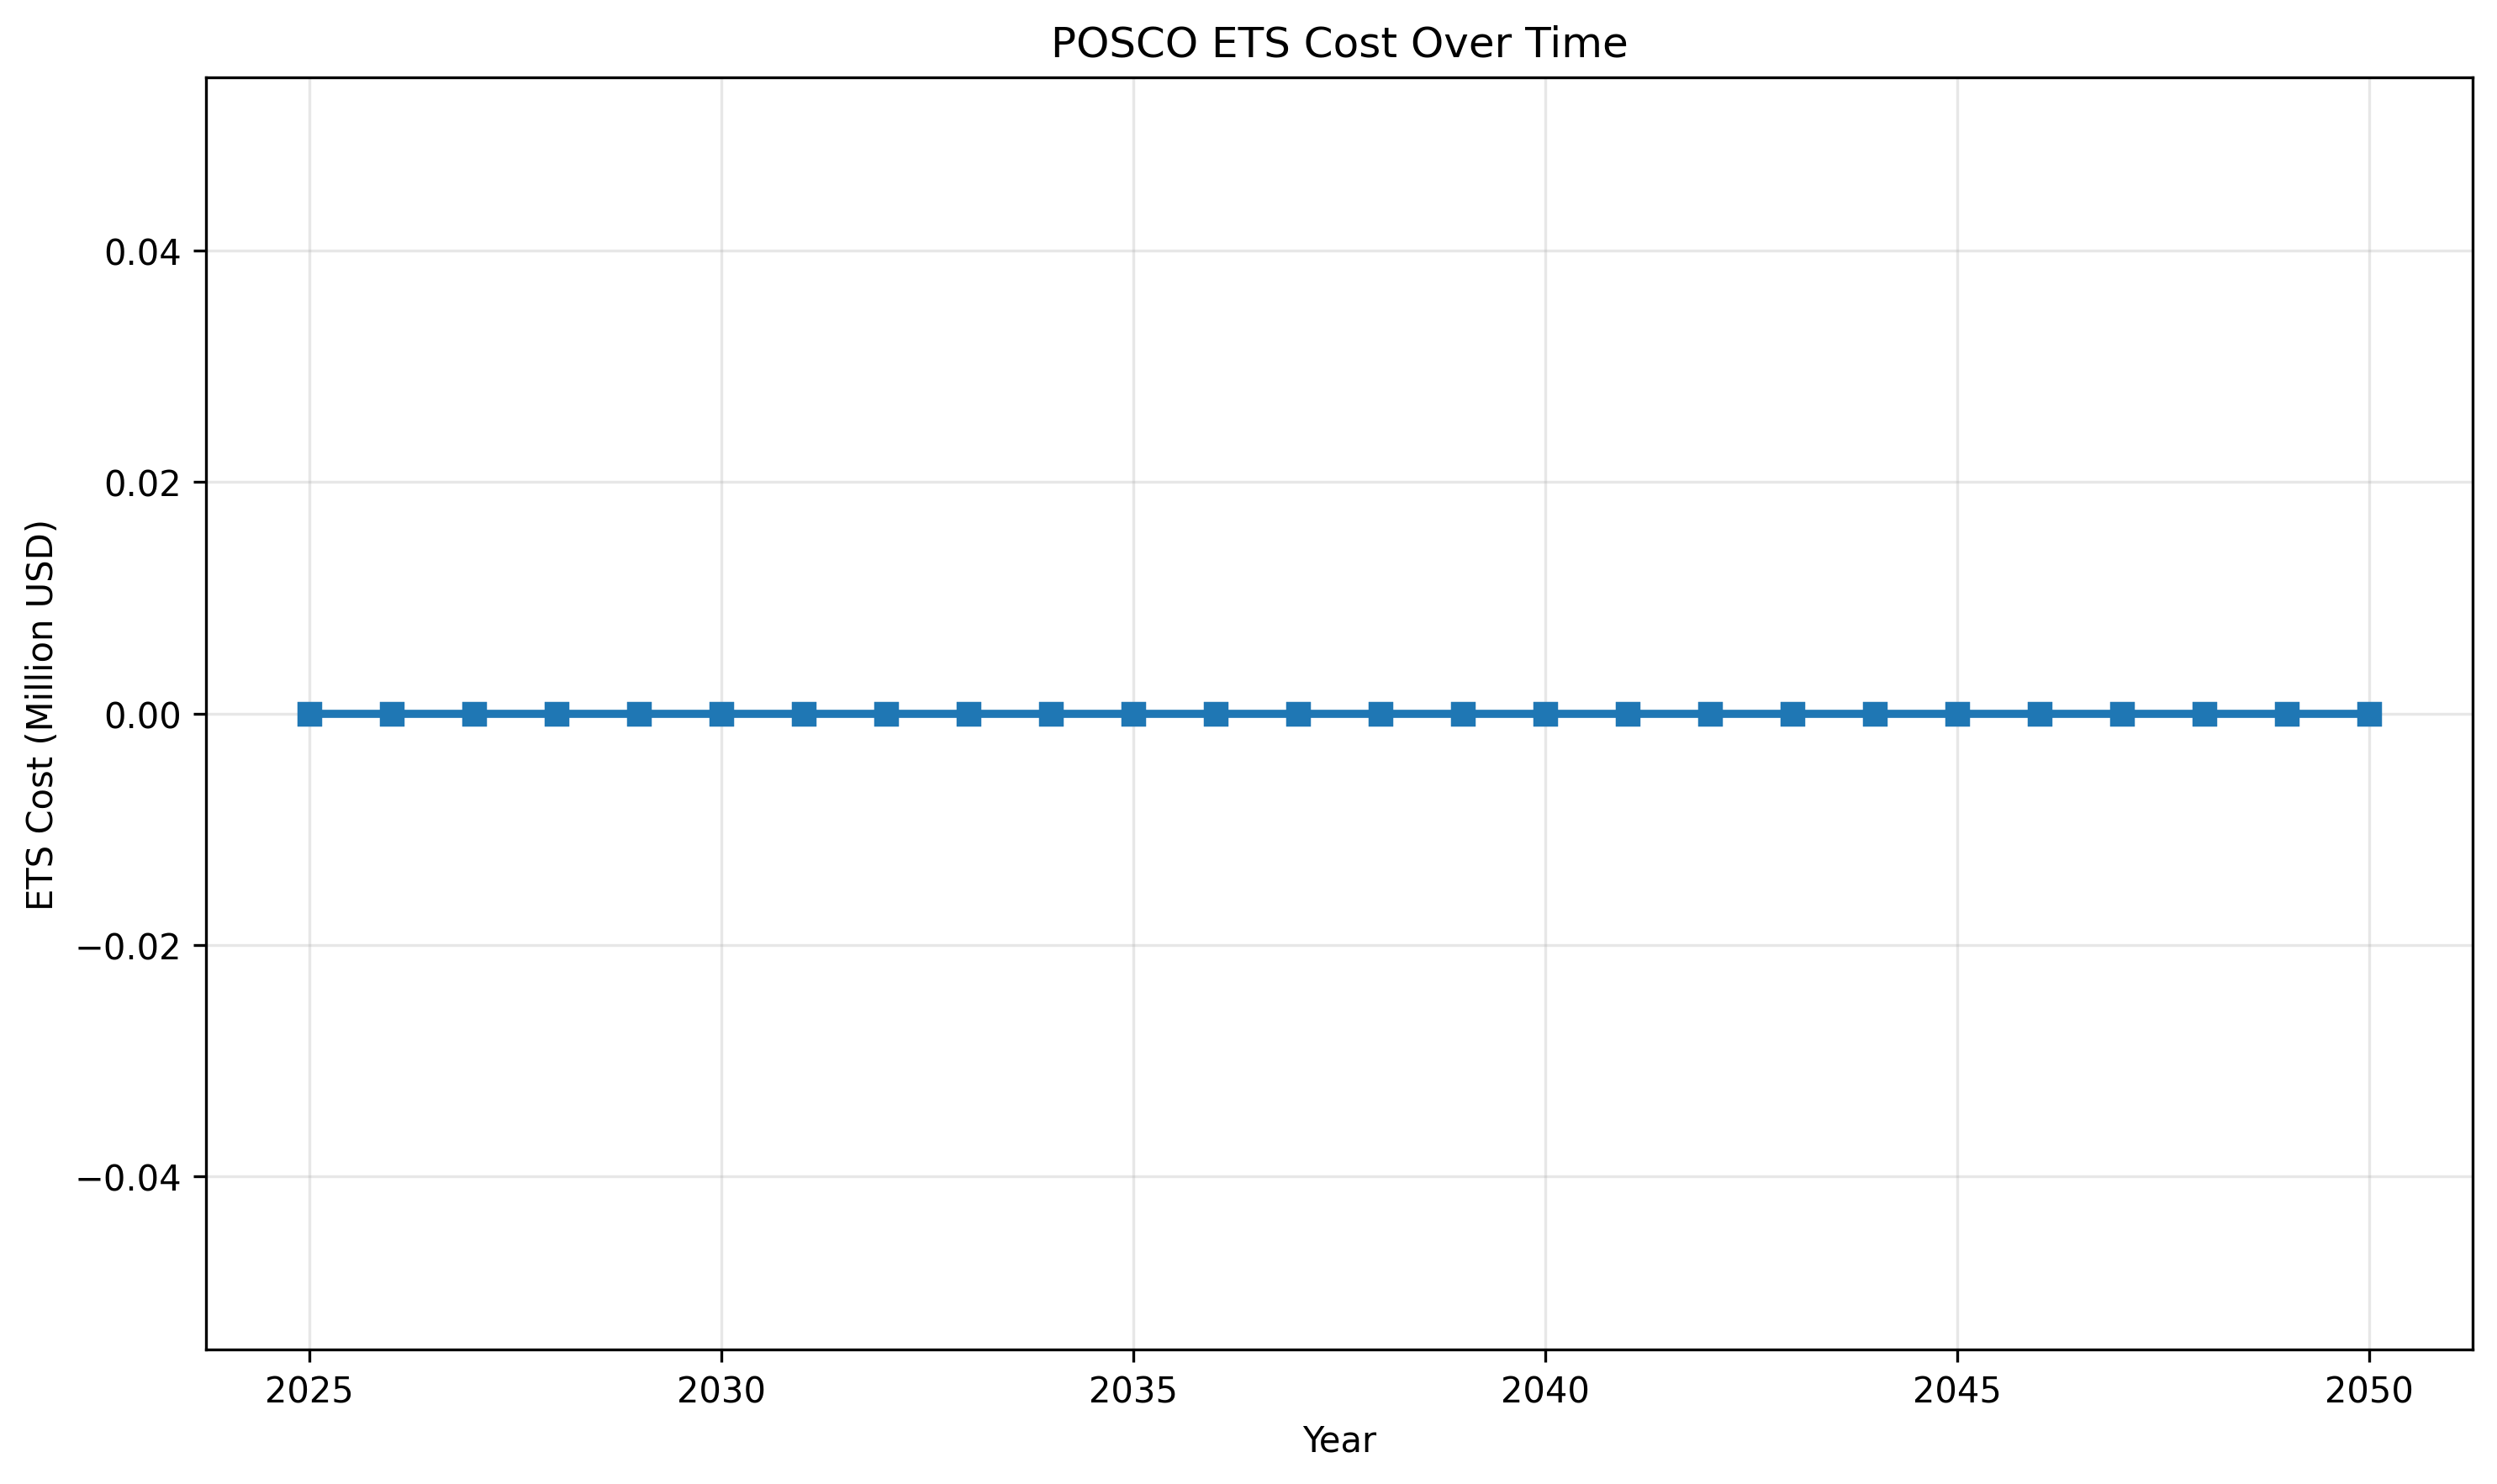
\includegraphics[width=0.8\linewidth]{ets_cost_by_scenario}
  \caption{Annual ETS compliance costs across the NGFS price trajectories plus the Net Zero 2050 (No CCUS) sensitivity.}
  \label{fig:ets-costs}
\end{figure}

Figure~\ref{fig:ets-costs} visualizes how compliance payments evolve over time. The NDC scenario shows persistently high annual ETS costs through 2050, peaking above \$3 billion/year in the mid-2040s as emissions remain high while allowance prices gradually rise. Net Zero pricing shows a different pattern: modest compliance costs through the late 2020s while free allocation remains generous, then a spike in the early 2030s as allocation tightens before CCUS retrofits come online, and finally a collapse to near-zero costs post-2035 as low-carbon technologies dominate the portfolio.

The policy implication is powerful: ambitious carbon pricing need not harm industrial competitiveness if it reaches levels sufficient to justify transformative investment. Half-measures that raise carbon prices modestly without crossing technology deployment thresholds create the worst of both worlds—firms face rising compliance costs without the price certainty needed to justify major capital commitments.

\subsection{CCUS unavailability quadruples carbon costs and forces expensive hydrogen adoption}

To test how critically our results depend on CCUS availability, we re-run the Net Zero 2050 price trajectory with carbon capture technology completely disabled (setting capture efficiency to zero). This sensitivity reveals stark trade-offs and highlights infrastructure dependencies that could derail decarbonization pathways.

Without CCUS, the technology portfolio shifts dramatically. Hydrogen-based direct reduction routes, which never appeared in the baseline scenarios, suddenly capture 35.7\% of production by 2050. Scrap-EAF remains capped at its feedstock-constrained maximum of 35.3\%, while unabated blast furnaces supply the remaining 29.0\% of output. The model has no choice but to turn to expensive hydrogen DRI because scrap availability is exhausted and conventional BF-BOF routes face prohibitive carbon costs without capture technology.

Yet the emission and cost outcomes deteriorate markedly compared to the CCUS-enabled pathway:

\begin{itemize}[leftmargin=*]
  \item Cumulative Scope 1 emissions climb to 1,324 MtCO$_2$, a +19\% increase versus the CCUS-enabled Net Zero case and a +19\% overshoot relative to the carbon budget.
  \item Annual emissions in 2050 settle at 29.0 MtCO$_2$, 26\% higher than the CCUS-enabled endpoint.
  \item Net ETS liabilities over the planning horizon jump from 72 MtCO$_2$ to 206 MtCO$_2$—nearly tripling.
  \item Cumulative ETS payments explode from \$9.3 billion to \$43 billion—more than quadrupling.
  \item Average steelmaking costs increase to \$815/t, eroding much of the competitiveness advantage delivered by CCUS-enabled pathways.
\end{itemize}

\begin{figure}[!t]
  \centering
  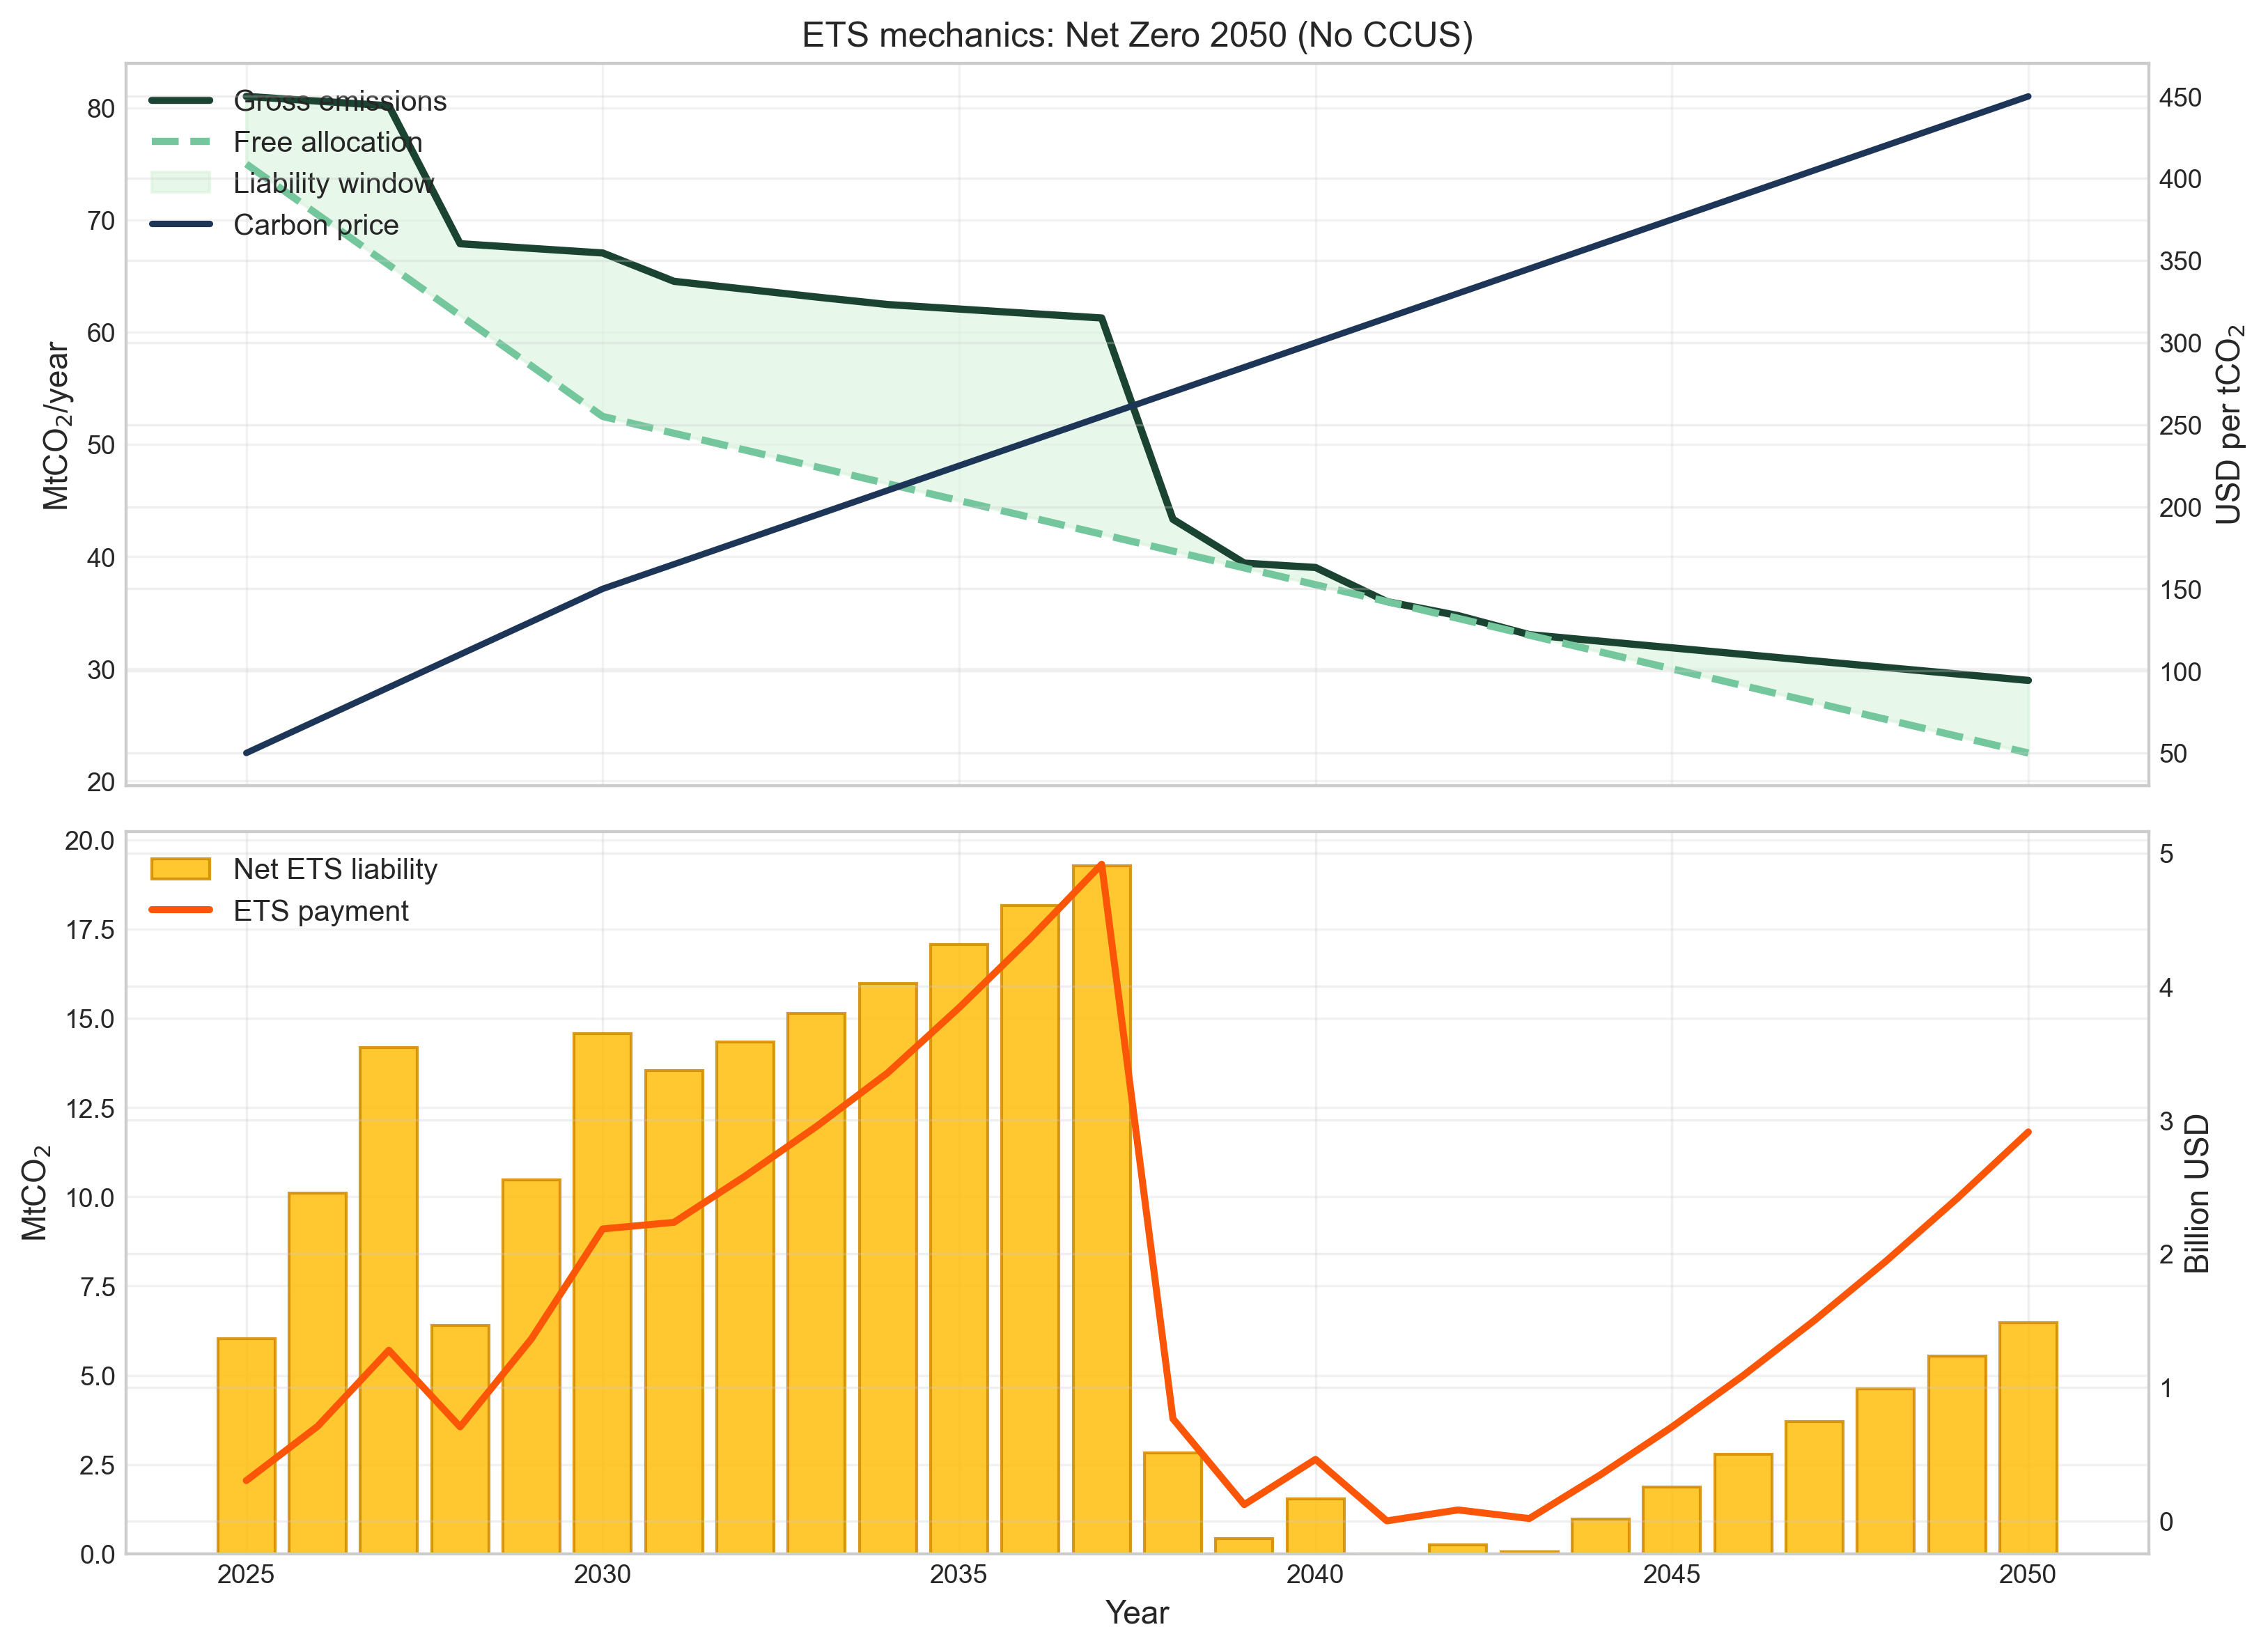
\includegraphics[width=0.85\linewidth]{ets_cost_logic}
  \caption{ETS cost mechanics for the Net Zero 2050 (No CCUS) pathway. The top panel contrasts gross emissions, free allocation, and allowance prices; the lower panel shows net ETS liabilities and resulting payments.}
  \label{fig:ets-logic}
\end{figure}

Figure~\ref{fig:ets-logic} illustrates the mechanism behind this cost explosion. The free allocation schedule declines steadily after 2030, but without CCUS technology to reduce gross emissions proportionally, a widening liability gap opens up. By the mid-2030s, net ETS liabilities exceed 5 MtCO$_2$/year. Combined with allowance prices crossing \$200-300/tCO$_2$, this generates multi-billion-dollar annual compliance payments that persist through 2050.

The No CCUS sensitivity underscores that hydrogen DRI adoption at current cost assumptions requires CCUS to absorb residual blast furnace output. Hydrogen alone cannot fully decarbonize the steel sector within realistic cost constraints—it needs CCUS as a complementary technology for transitional blast furnace operations. Without a credible CCUS program backed by CO$_2$ transport and storage infrastructure, the ETS would shoulder far larger compliance volumes, the carbon budget gap would remain unacceptably wide, and competitiveness would erode substantially.

This finding has crucial policy implications: Korea cannot simply choose between "green hydrogen" and "CCUS" as alternative decarbonization strategies. The cost-optimal pathway requires both—scrap-EAF where feedstock allows, CCUS retrofits for transitional blast furnace operations, and hydrogen DRI only for remaining capacity after exhausting cheaper options. Industrial policy that favors one technology over others risks missing this complementarity and driving suboptimal, expensive outcomes.

\subsection{Hydrogen cost breakthroughs alone cannot close the policy-performance gap}

To test whether lower hydrogen costs could fundamentally change technology choices and budget compliance, we conducted sensitivity analysis using alternative hydrogen price trajectories. The repository includes three scenarios (\texttt{outputs/h2\_breakthrough}, \texttt{h2\_optimistic}, and \texttt{h2\_zero}) that progressively reduce delivered hydrogen costs below our baseline assumptions.

The results are striking in their consistency. Even lowering hydrogen prices from the baseline \$4.5/kg to a "breakthrough" trajectory reaching \$2.5/kg by 2035—representing dramatic cost reductions from advanced electrolyzer deployment and cheap renewable electricity—barely shifts the technology mix under Net Zero pricing. Scrap-EAF rises modestly to 46\% of 2050 output (up from 36\% in baseline), CCUS-backed blast furnaces decline to 38\% (down from 51\%), and hydrogen DRI captures just 16\% of production rather than remaining at zero.

Cumulative emissions in this breakthrough hydrogen case reach 1,188 MtCO$_2$—essentially unchanged from the baseline 1,190 MtCO$_2$. Lifetime system costs shift by less than \$1.5 billion out of \$791 billion total, a rounding error. The carbon budget overshoot persists at +7.0\%, and policy implications remain identical.

We pushed this analysis to an extreme "zero-cost hydrogen" stress test where hydrogen is provided for free. Even under this utterly unrealistic assumption, cumulative emissions decline only to 1,175 MtCO$_2$—still overshooting the budget by +5.9\%. Why? Because capital intensity, ore quality constraints, and scrap availability ceilings—rather than hydrogen molecule prices alone—govern technology choices. Building hydrogen DRI facilities requires \$1,500/tpy in capital investment compared to \$800/tpy for conventional blast furnaces. Moreover, hydrogen DRI production requires high-quality direct-reduced iron pellets rather than standard iron ore fines, introducing feedstock constraints that limit hydrogen route expansion regardless of H$_2$ prices.

These sensitivities confirm that policy packages aimed solely at subsidizing hydrogen production would leave the carbon budget gap essentially intact unless paired with infrastructure investments that tackle non-price barriers: pellet production facilities for DRI feedstock, hydrogen pipeline networks and storage, and guaranteed off-take contracts that de-risk large capital commitments. The sobering conclusion is that simply making green hydrogen cheap will not transform the steel sector—the binding constraints lie elsewhere.

Table~\ref{tab:scenario-comparison} consolidates these findings across all scenarios and sensitivities, providing a comprehensive reference for comparing emission outcomes, technology choices, costs, and budget gaps.
